\subsection{Preparación de ejemplos y predicción autorregresiva}
\label{sec:sft-ejemplos}
Antes de entrenar, cada ejemplo se transforma en una secuencia de tokens mediante el tokenizador del modelo. En un formato conversacional, una plantilla organiza las instrucciones y los mensajes e incorpora delimitadores de roles, por lo que deben respetarse las convenciones del modelo de partida. Si $T_i$ es la longitud de la respuesta $i$, su probabilidad se descompone en predicciones del token siguiente,
\begin{equation}
p_\theta(y_i\mid x_i)=\prod_{t=1}^{T_i}
p_\theta(y_{i,t}\mid x_i,y_{i,<t}),
\label{eq:sft-autorregresivo}
\end{equation}
donde $\theta$ representa los parámetros del modelo y $y_{i,<t}$ contiene los tokens anteriores de la respuesta. Esta distribución es la que, en la sección~\ref{sec:marco-rl}, se interpretará como política y se denotará por $\pi_\theta$.

Durante el entrenamiento se aplica teacher forcing, una técnica que utiliza los tokens anteriores de la respuesta de referencia como contexto para predecir el siguiente token. En cada posición, el modelo recibe la consulta y la parte de la referencia que precede al token esperado, y la pérdida compara la distribución que produce con ese token correcto. Así, aunque asigne mayor probabilidad a un token incorrecto, las predicciones siguientes siguen utilizando el historial de la referencia. En cambio, durante la generación, el contexto se amplía con los tokens que el propio modelo va produciendo, de modo que un error puede influir en las predicciones posteriores.

Como la referencia completa está disponible durante el entrenamiento, un Transformer causal puede calcular las predicciones de distintas posiciones en paralelo, utilizando una máscara de atención que impide acceder a los tokens futuros~\cite{vaswani2017attention}. La figura~\ref{fig:sft-secuencia} muestra cómo se organizan el contexto, la respuesta y el relleno, distinguiendo qué información utiliza el modelo de qué posiciones se supervisan.

\begin{figure}[htbp]
\centering
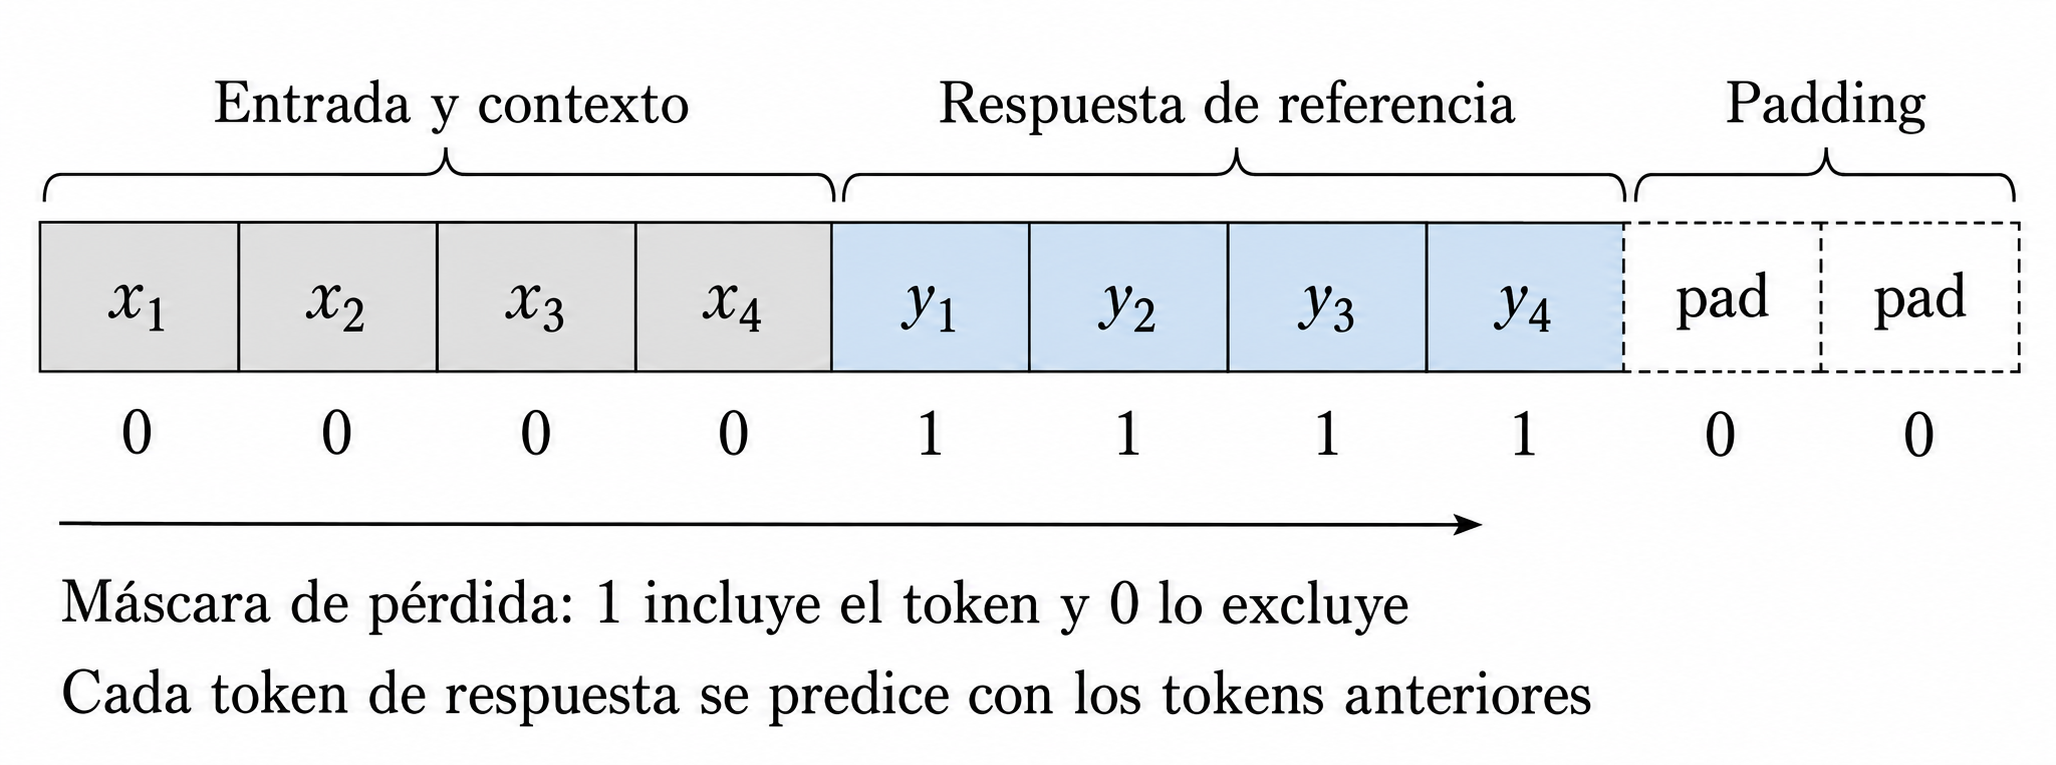
\includegraphics[width=0.95\textwidth]{Figuras/02-marco-teorico/02-ajuste-supervisado/sft-secuencia-tokens.png}
\caption{Secuencia de tokens con pérdida calculada únicamente sobre la respuesta.}
\label{fig:sft-secuencia}
\end{figure}

La preparación también requiere separar entrenamiento y validación, comprobar duplicados y evitar que una misma consulta o una variante cercana aparezca en ambos conjuntos. Asimismo, el límite de secuencia comprende la entrada y la respuesta, por lo que el truncamiento puede eliminar contexto o contenido supervisado y debe registrarse como parte del procedimiento. Este límite difiere de la cantidad máxima de tokens nuevos que se permite generar durante la inferencia, mientras que el padding permite reunir secuencias de longitudes distintas en un batch y se excluye de la pérdida para que el relleno no se aprenda como respuesta.

